% vim: set ft=tex :

% vim: set ft=tex tabstop=4 shiftwidth=4 noexpandtab:

% opening %{{{1

\documentclass[tikz, border=1mm]{standalone}

% packages and libraries %{{{1

% ---- not necessary since the documentclass[tikz ...] requires it automatically
% \usepackage{tikz}

\usepackage{../../include/latex/tex/custom}

\usetikzlibrary{calc,intersections,angles,quotes,shapes.geometric,arrows.meta,decorations.markings}

\usepackage{tkz-euclide}

% colors %{{{1

\definecolor{goldenbrown}{HTML}{5b3c11}

%\definecolor{somebrown}{RGB}{101,67,33}

%\colorlet{somebrown}{brown!80!black}

% style %{{{1

\tikzset{
	% ------- every something
	every picture/.style={
		scale=1.0,
	},
	every coordinate/.style={
		fill=black, circle, inner sep=1pt,
	},
	every path/.style={
		line width=0.3pt,
	},
	every node/.style={
		font=\normalsize,
	},
	every angle/.style={
	},
	every pic/.style={
		% ---- does not work
		%draw,
		%-{Straight Barb[length=1.2mm]},
	},
	% ------- custom
	vector/.style={
		-{Straight Barb[length=1.2mm]},
		%thick,
	},
	double arrow/.style={
		{Straight Barb[length=1.2mm]}-{Straight Barb[length=1.2mm]},
	},
	mid arrow/.style={
		postaction={
			decorate,
			decoration={
				markings,
				mark=at position #1 with {
					\arrow{Straight Barb[length=1.2mm]}
				}
			}
		}
	},
	mid arrow/.default=0.5,
	construction/.style={
		line width=0.1pt,
		dashed,
	},
	dimension/.style={
		line width=0.2pt,
		<->,
		goldenbrown,
	},
	dimension extension/.style={
		line width=0.2pt,
		dashed,
		goldenbrown,
	},
}


% opening %{{{1

\begin{document}
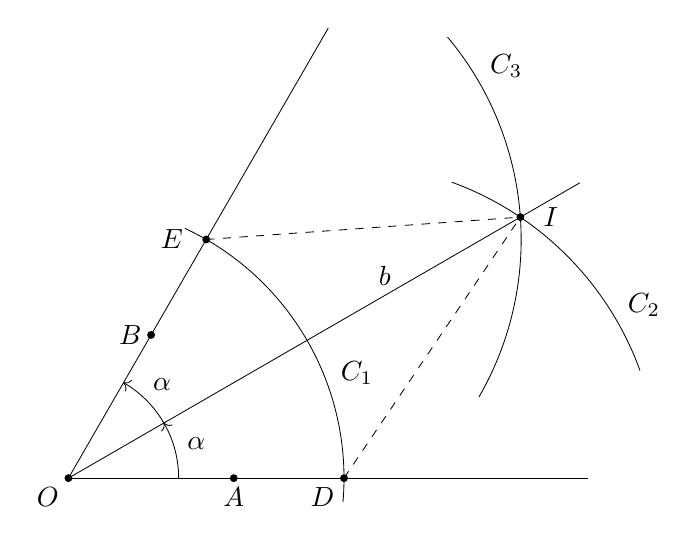
\begin{tikzpicture}[scale=1.0]

% parameters %{{{1

	\def\len{2.1}
	\def\extlen{3}
	\def\radius{3.5}
	\def\arcradius{4}
	\def\ang{60}

% coordinates %{{{1

	\coordinate (O) at (0,0);
	\coordinate (A) at (0:\len);
	\coordinate (B) at (\ang:\len);

% coordinates of points in circles %{{{2

	\coordinate (R) at ($(O) + (\radius, 0)$);

% intersections %{{{1

	\tkzInterLC(O,A)(O,R)\tkzGetSecondPoint{D}
	\tkzInterLC(O,B)(O,R)\tkzGetSecondPoint{E}

	\begin{pgfinterruptboundingbox}
		\path[name path=circleA] (D) circle (\arcradius);
		\path[name path=circleB] (E) circle (\arcradius);
		\path [name intersections={of=circleA and circleB, by={I,J}}];
	\end{pgfinterruptboundingbox}

% vectors %{{{1

	\coordinate (v1) at ($ (A) - (O) $);
	\coordinate (v2) at ($ (B) - (O) $);
	\coordinate (v3) at ($ (I) - (O) $);

% unit vectors %{{{2

	\coordinate (u1) at ($ (0,0)!1cm!(v1) $);
	\coordinate (u2) at ($ (0,0)!1cm!(v2) $);
	\coordinate (u3) at ($ (0,0)!1cm!(v3) $);

% coordinates from vectors %{{{1

	\coordinate (X) at ($ (A) + {1.5*\extlen}*(u1) $);
	\coordinate (Y) at ($ (B) + {1.5*\extlen}*(u2) $);
	\coordinate (Z) at ($ (O) + {2.5*\extlen}*(u3) $);

% segments %{{{1

	\draw (O) -- (X);
	\draw (O) -- (Y);
	\draw (O) -- (Z);

	\draw[dashed] (D) -- (I);
	\draw[dashed] (E) -- (I);

% circles %{{{1

	%\draw (O) circle (\radius);

% circular arcs %{{{1

	\draw (O) ++(-5:\radius) arc (-5:{\ang + 5}:\radius);

	\draw (D) ++(20:\arcradius) arc (20:70:\arcradius);
	\draw (E) ++(-30:\arcradius) arc (-30:40:\arcradius);

% thick vertices %{{{1

	\fill (O) circle (0.5mm);
	\fill (A) circle (0.5mm);
	\fill (B) circle (0.5mm);
	\fill (D) circle (0.5mm);
	\fill (E) circle (0.5mm);
	\fill (I) circle (0.5mm);

% vertices labels %{{{1

	\node[below left] at (O) {$O$};
	\node[below] at (A) {$A$};
	\node[left] at (B) {$B$};
	\node[below left] at (D) {$D$};
	\node[label={[label distance=0.5mm]left:$E$}] at (E) {};
	\node[label={[label distance=0.5mm]right:$I$}] at (I) {};

% segments labels %{{{1

	\node[above] at ($ (O)!0.7!(I) $) {$b$};

% circular arcs labels %{{{1

	\node at ($ (O)+(20:\radius+0.4) $) {$\mathscr{C}_1$};
	\node at ($ (D)+(30:\arcradius+0.4) $) {$\mathscr{C}_2$};
	\node at ($ (E)+(30:\arcradius+0.4) $) {$\mathscr{C}_3$};

% angles labels %{{{1

	\pic[draw, ->, "$\alpha$", angle radius=1.4cm, angle eccentricity=1.2]
	{angle = A--O--I};

	\pic[draw, ->, "$\alpha$", angle radius=1.4cm, angle eccentricity=1.2]
	{angle = I--O--B};

% closing %{{{1

\end{tikzpicture}
\end{document}
